\chapter{Analysis Selection}
\label{chap:bbbb-selection}

\section{Analysis Selection}
\label{sec:analysis-selection}
After the trigger selections of Section \ref{sec:trigger}, a variety of selections on the analysis objects
are made, with the goal of (1) reconstructing a $HH$-like topology and (2) suppressing contributions from 
background processes. 

Both analyses begin with a common pre-selection, requiring at least four $R=0.4$ anti-$k_{T}$ jets with 
$|\eta| < 2.5$ and $p_{T} > \SI{40}{\GeV}$. The $|\eta| < 2.5$ requirement is necessary for $b$-tagging
due to the coverage of the ATLAS tracking detector (see Chapter \ref{chap:experiment}), 
while the $p_{T} > \SI{40}{\GeV}$ requirement is motivated by the trigger thresholds. A low $p_{T}$ category, 
which would include events failing the analysis selection due to this $p_{T}$ cut, 
was considered for the non-resonant search, but was found to contribute minimal sensitivity.
At least two of the jets passing this pre-selection are required to be $b$-tagged, and additional $b$-tagging 
requirements are made to define the following regions:
\begin{itemize}
	\item ``2$b$ Region'': require exactly two $b$-tagged jets, used for background estimation
	\item ``4$b$ Region'': require at least (but possibly more) four $b$-tagged jets, used as a signal
	region for both resonant and non-resonant searches
\end{itemize}

The non-resonant analysis additionally defines two $3b$ regions:
\begin{itemize}
	\item ``3$b$+1 loose Region'': require exactly three $b$-tagged jets which 
	pass the 77~\% b-tagging working point (nominal) and one additional jet that fails the  
	77~\% b-tagging working point but passes the \emph{looser} 85~\% b-tagging working point. Used 
	as a signal region for the non-resonant search.
	\item ``3$b$+1 fail Region'': complement of 3$b$+1 loose. Require exactly three $b$-tagged jets 
	which pass the 77~\% b-tagging working point, but require that none of the remaining jets pass 
	the 85~\% b-tagging working point. Used as a validation region for the non-resonant search.
\end{itemize}
After these requirements, four jets are chosen, ranked first by $b$-tagging requirement and then 
by $p_{T}$ (e.g. for the 2$b$ region, the jets chosen are the two $b$-tagged jets and the two 
highest $p_{T}$ non-tagged jets; for the $4b$ region, the jets are the four highest $p_{T}$ $b$-tagged
jets). To match the topology of a $HH\rightarrow \bbbb$ event, these four jets are then \emph{paired}
into \emph{Higgs candidates}: the four jets are split into two sets of two, and each of these pairs is
used to define a reconstructed object that is a proxy for a Higgs in a $HH$ event. The four-vectors of 
these reconstructed objects may then be used for a variety of selections which check the consistency 
of the reconstructed $HH$ system with the expected $HH$ signal kinematics. Kinematic quantities corresponding 
to each Higgs candidate are denoted with subscripts $H1$ and $H2$ for leading and subleading Higgs candidates 
respectively (e.g. $m_{H1}$ and $m_{H2}$ for the Higgs candidate masses).

For four jets there are three possible pairings of jets into Higgs candidates. For signal events, a correct 
pairing can be identified
(provided all necessary jets pass pre-selection) using the truth information of the Monte Carlo simulation, 
and such information may be used to design/select an appropriate pairing algorithm. This is only part of 
the story, however. The vast majority of the events in data do \emph{not} include a real $HH$ decay (this is 
a search for a reason!), either because the event originates from a background process (e.g. for $4b$ events), or 
because the selection is not designed to maximize the signal (e.g. $2b$ events). As the pairing is 
part of the selection, it must still be run on such events, such that various algorithms which achieve similar
performance in terms of pairing efficiency may have vastly different impacts in terms of the shape of the background
and the biases inherent in the background estimation procedure. The interplay between these two facets of the 
pairing is an important part of the choices made for this analysis.

A comparison of different shapes due to three different paring strategies is shown in
Figure \ref{fig:pairing-massplanes}. The Boosted Decision Tree (BDT) pairing and $\min{\dr}$ pairing 
are used for the analyses presented here, and are described in more detail below. The $D_{HH}$ pairing 
was used for the early Run 2 searches~\cite{EXOT-2016-31}, and is based on minimizing the quantity 
\begin{equation}
D_{HH} = \frac{\qty|m_{H1} - \frac{120}{110}m_{H2}|}{\sqrt{1+\qty(\frac{120}{110})^2}},
\end{equation}
corresponding to the the distance of the reconstructed Higgs candidate masses from a line 
running from $(0, 0)$ to the center of the signal region, (\SI{120}{\GeV}, \SI{110}{\GeV}) in 
leading and subleading Higgs candidate masses, ($m_{H1}$, $m_{H2}$). Note that while 
this achieves good pairing efficiency with respect to truth across a broad $HH$ mass range, it significantly 
sculpts the mass plane (as seen in Figure \ref{fig:pairing-massplanes}), motivating the new 
approaches considered here.


\begin{figure}[ht]
\centering
\subfloat[BDT pairing]{\label{fig:BDT-massplane}
		  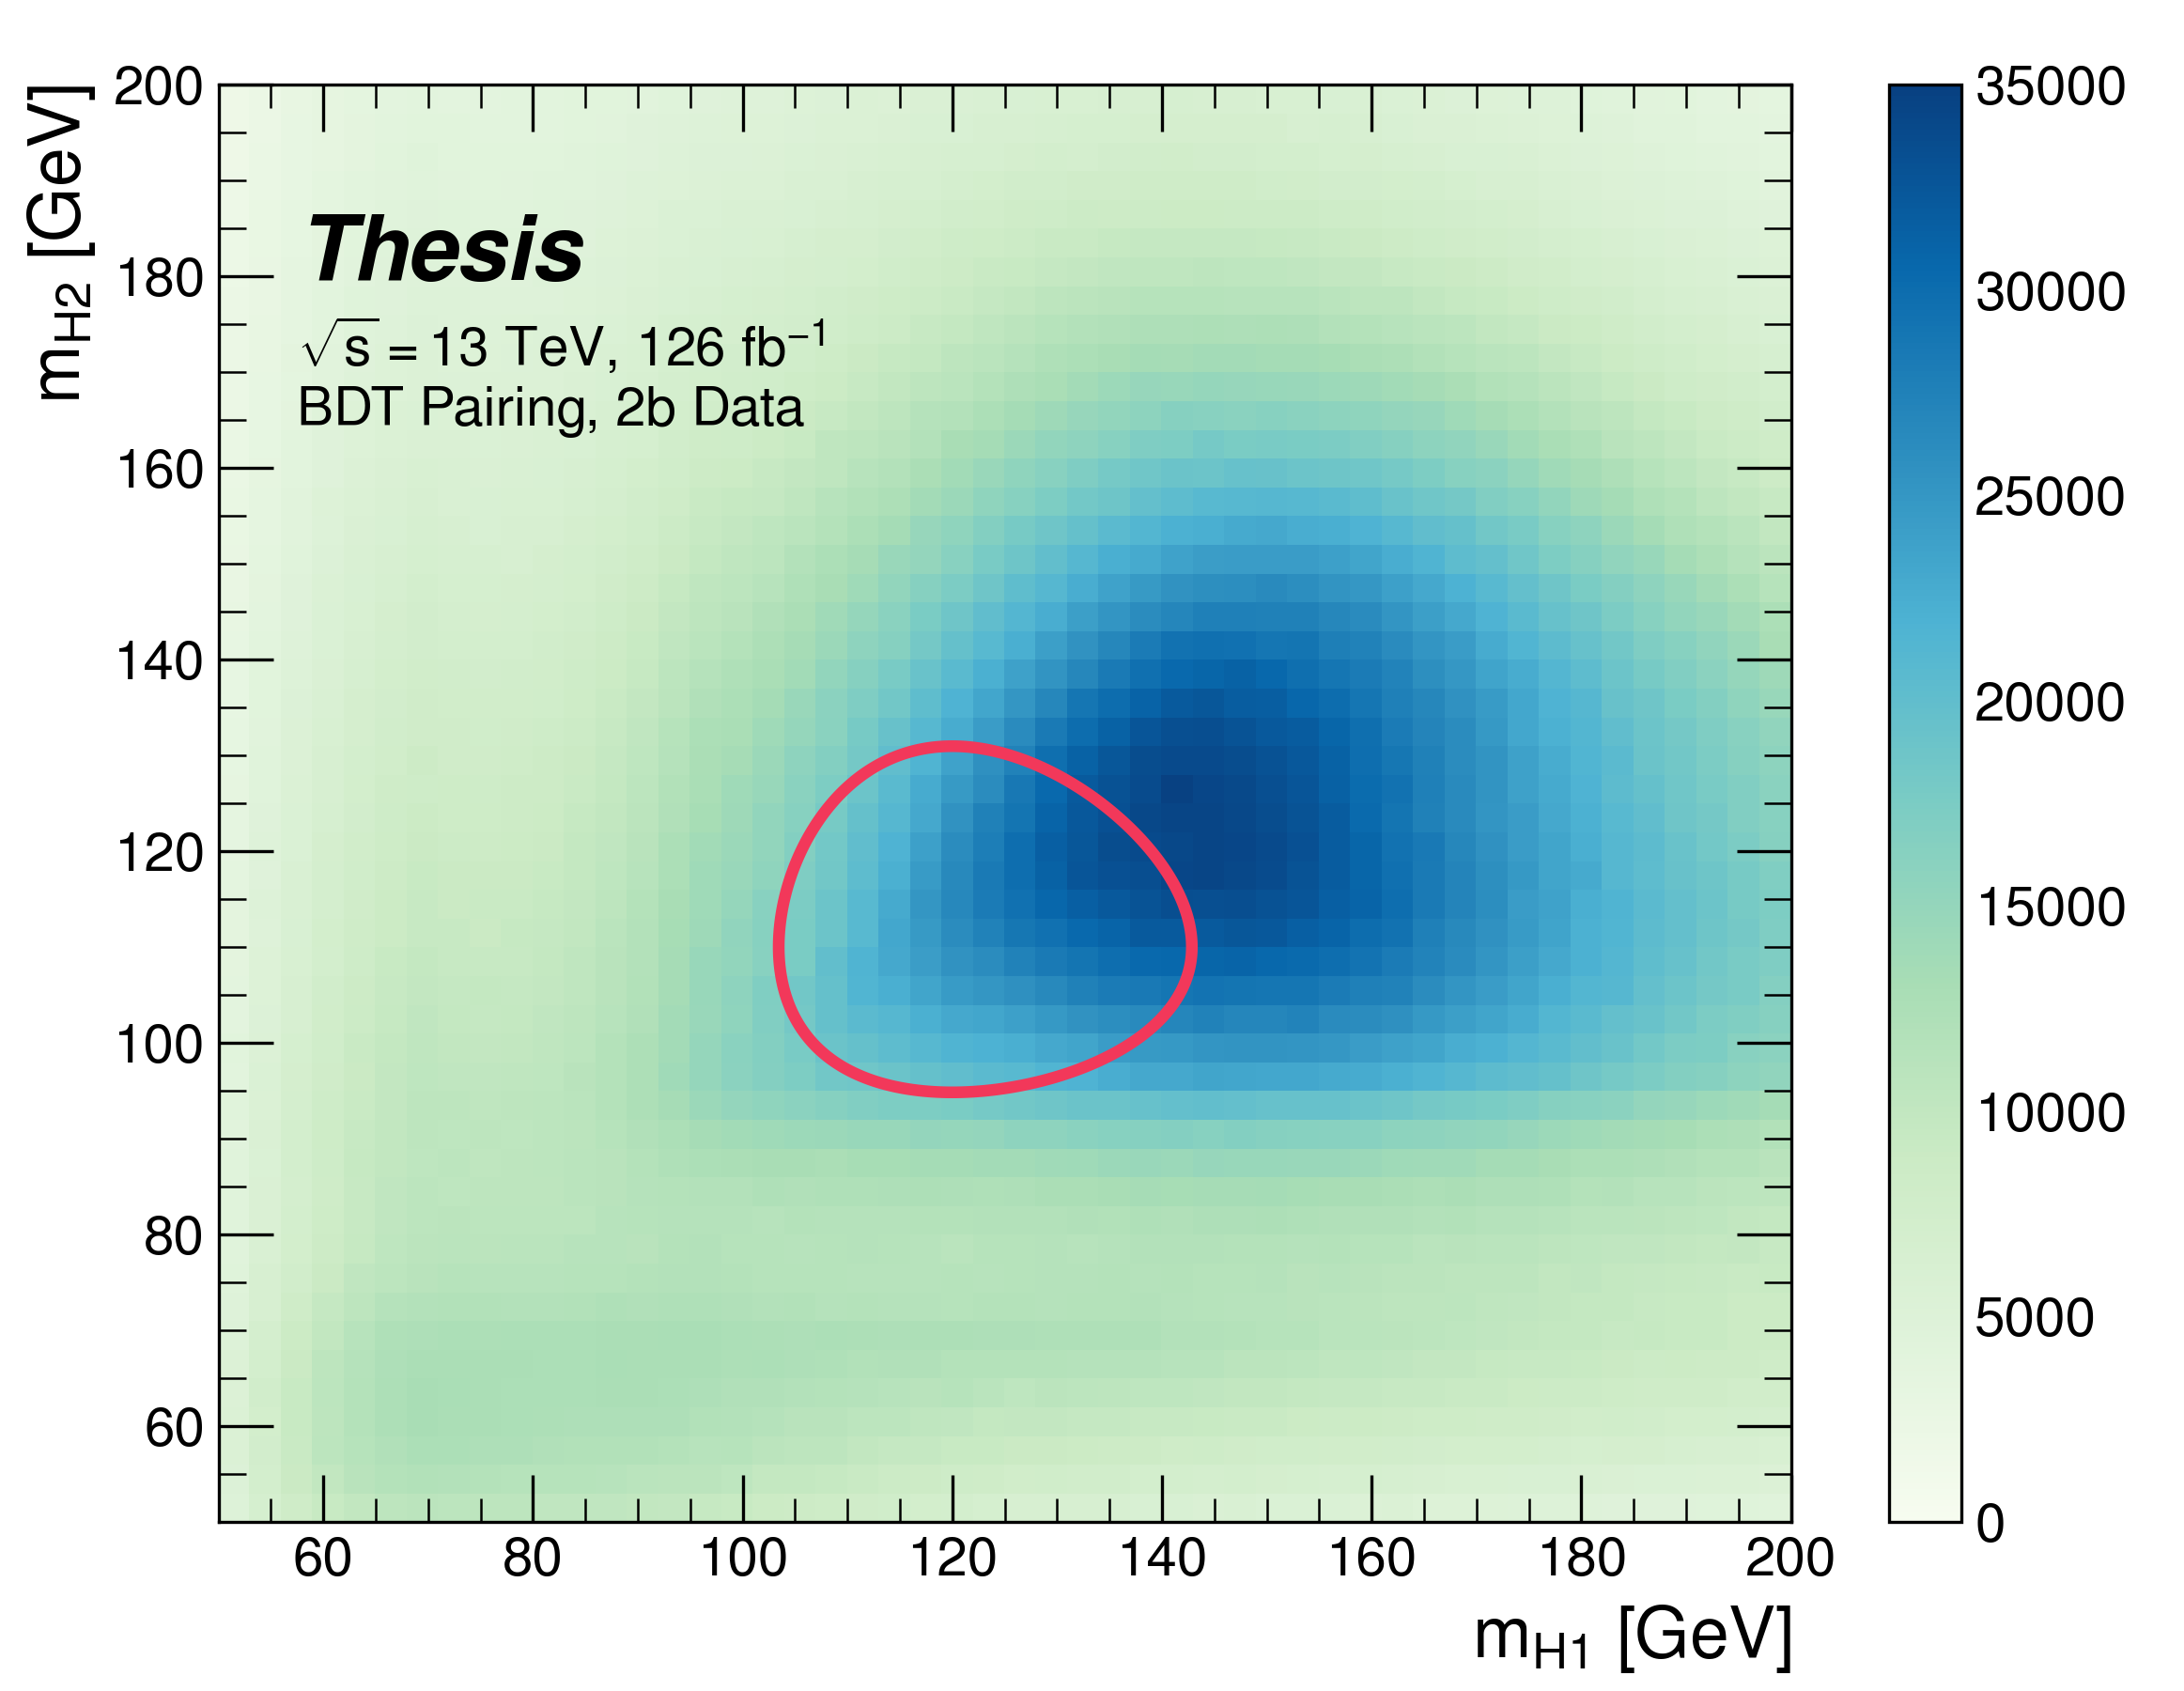
\includegraphics[width=0.48\textwidth]{figures/BDT-pairing-2b-massplane.png}
		 }
\subfloat[$\min\Delta R$ pairing]{\label{fig:mindR-massplane}
		  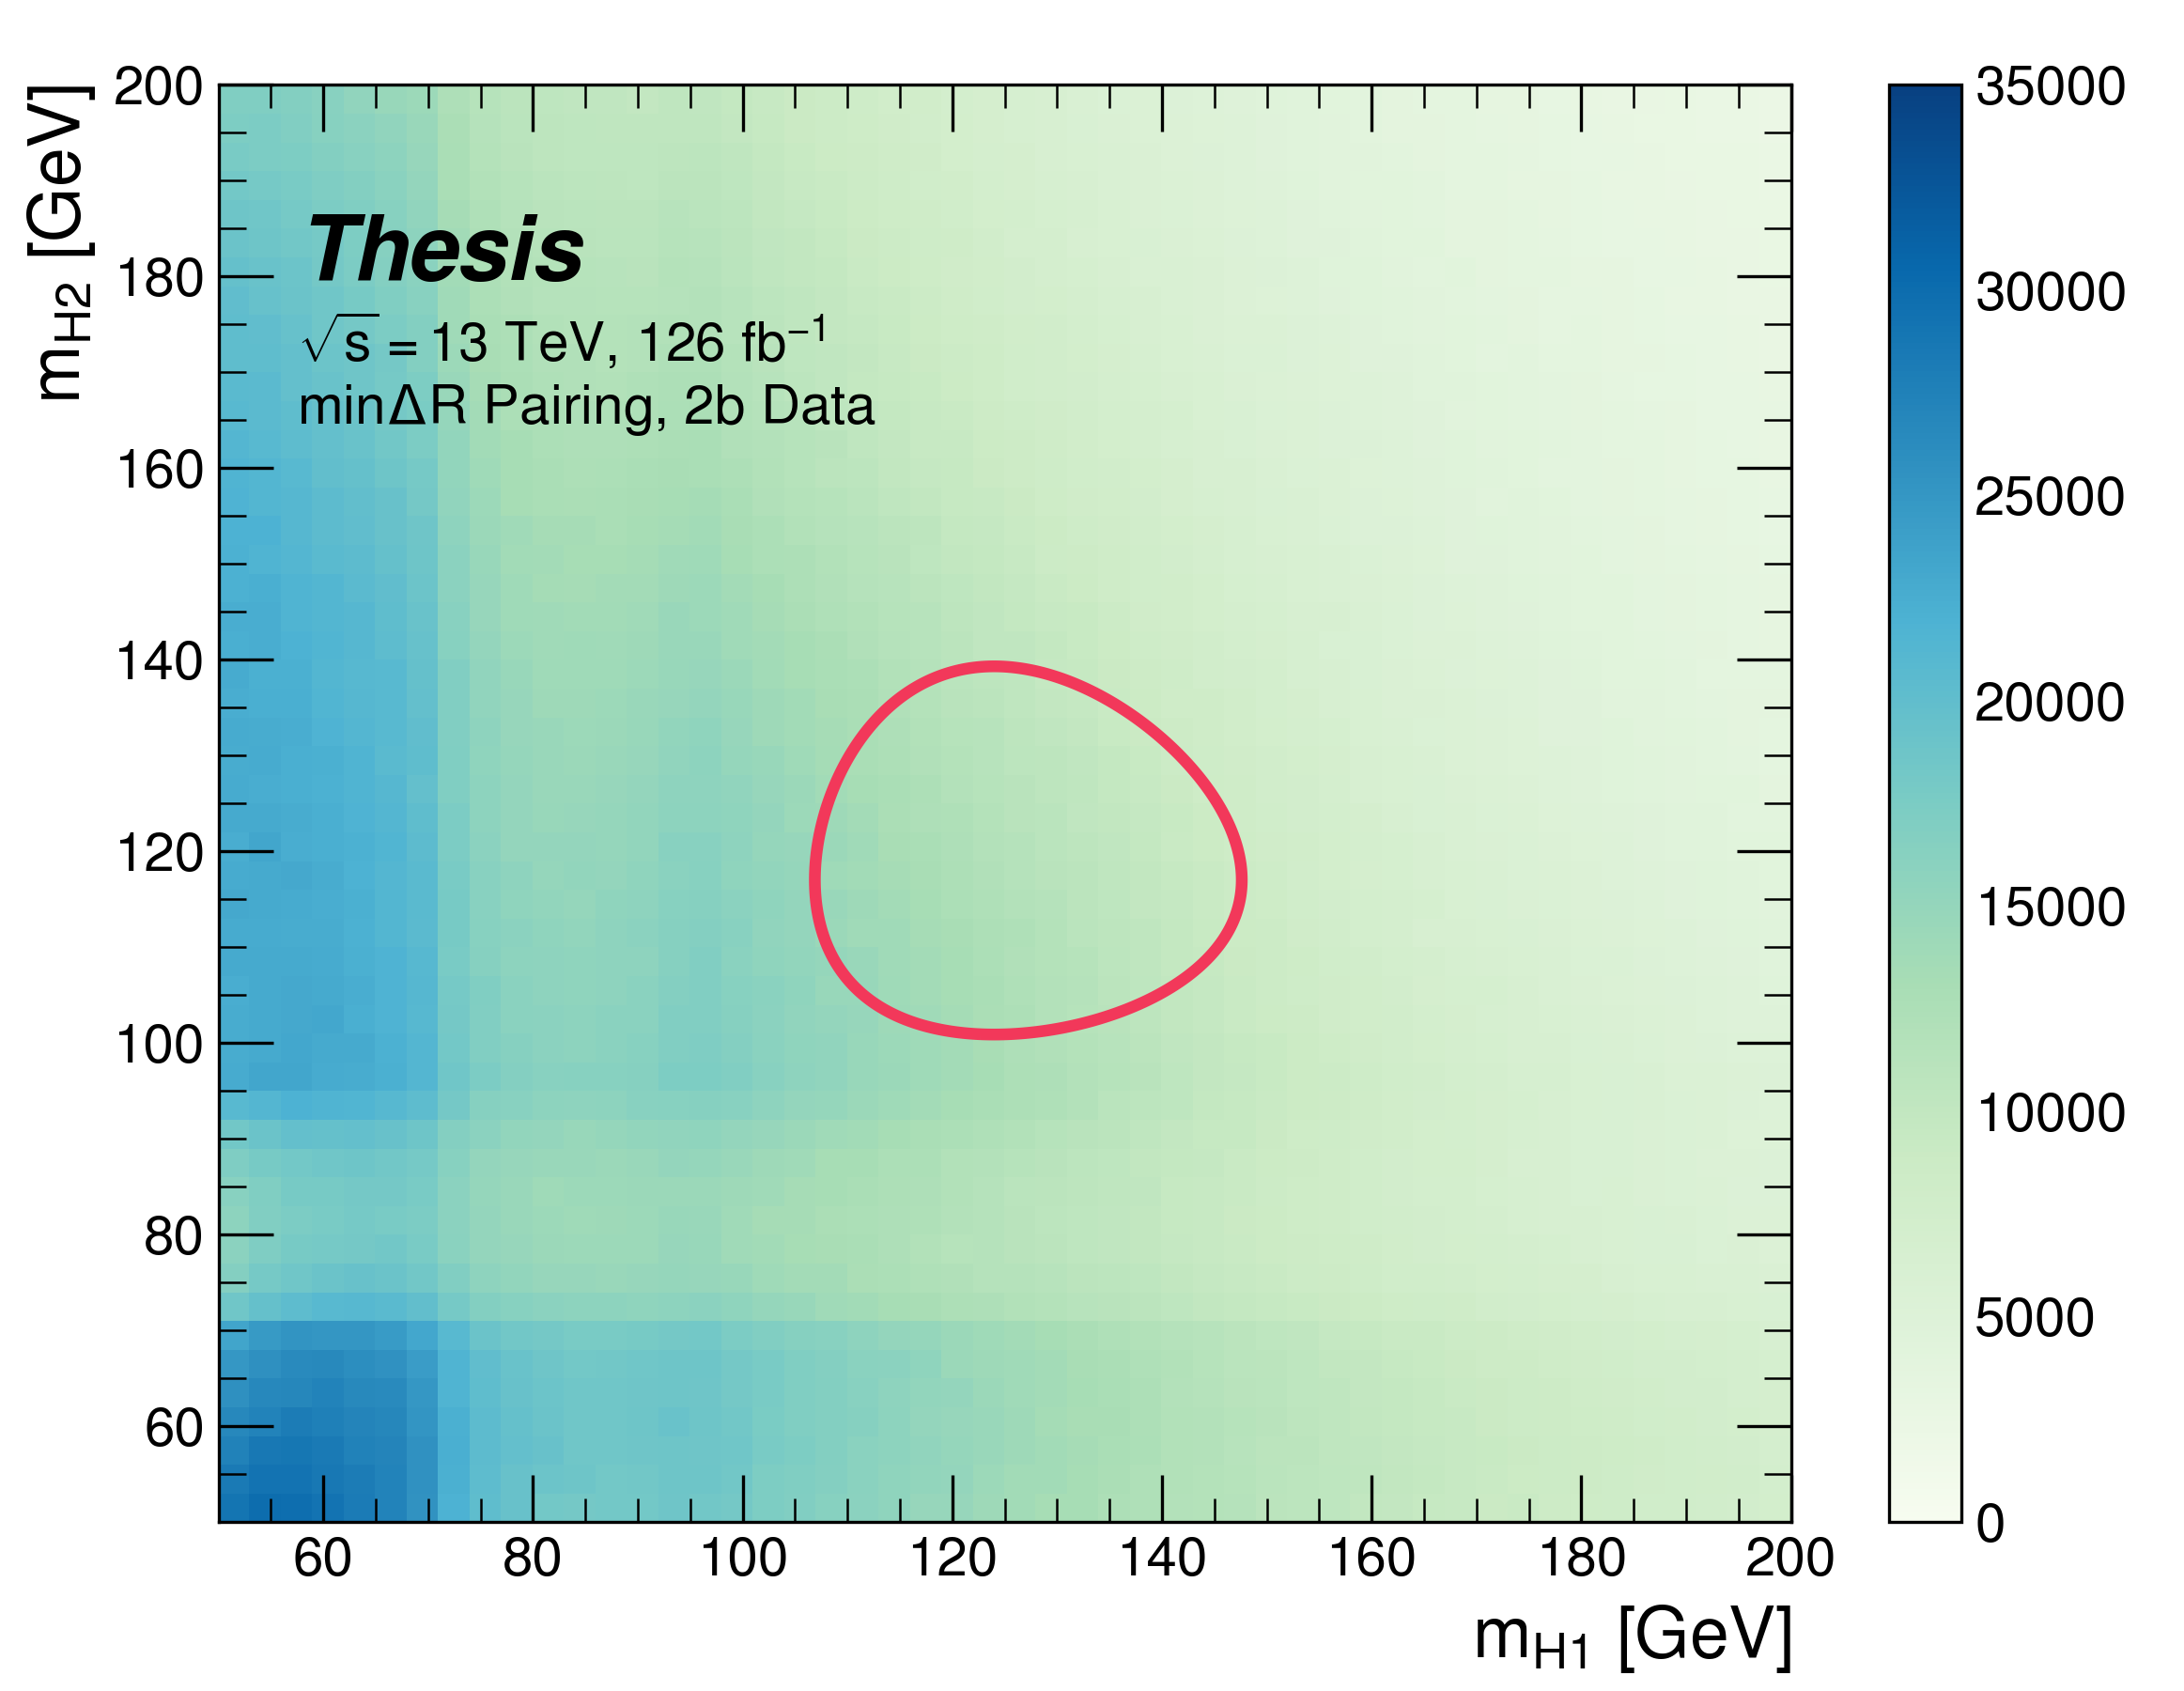
\includegraphics[width=0.48\textwidth]{figures/mindR-pairing-2b-massplane.png}
		 }

\subfloat[$D_{HH}$ pairing]{\label{fig:DHH-massplane}
		  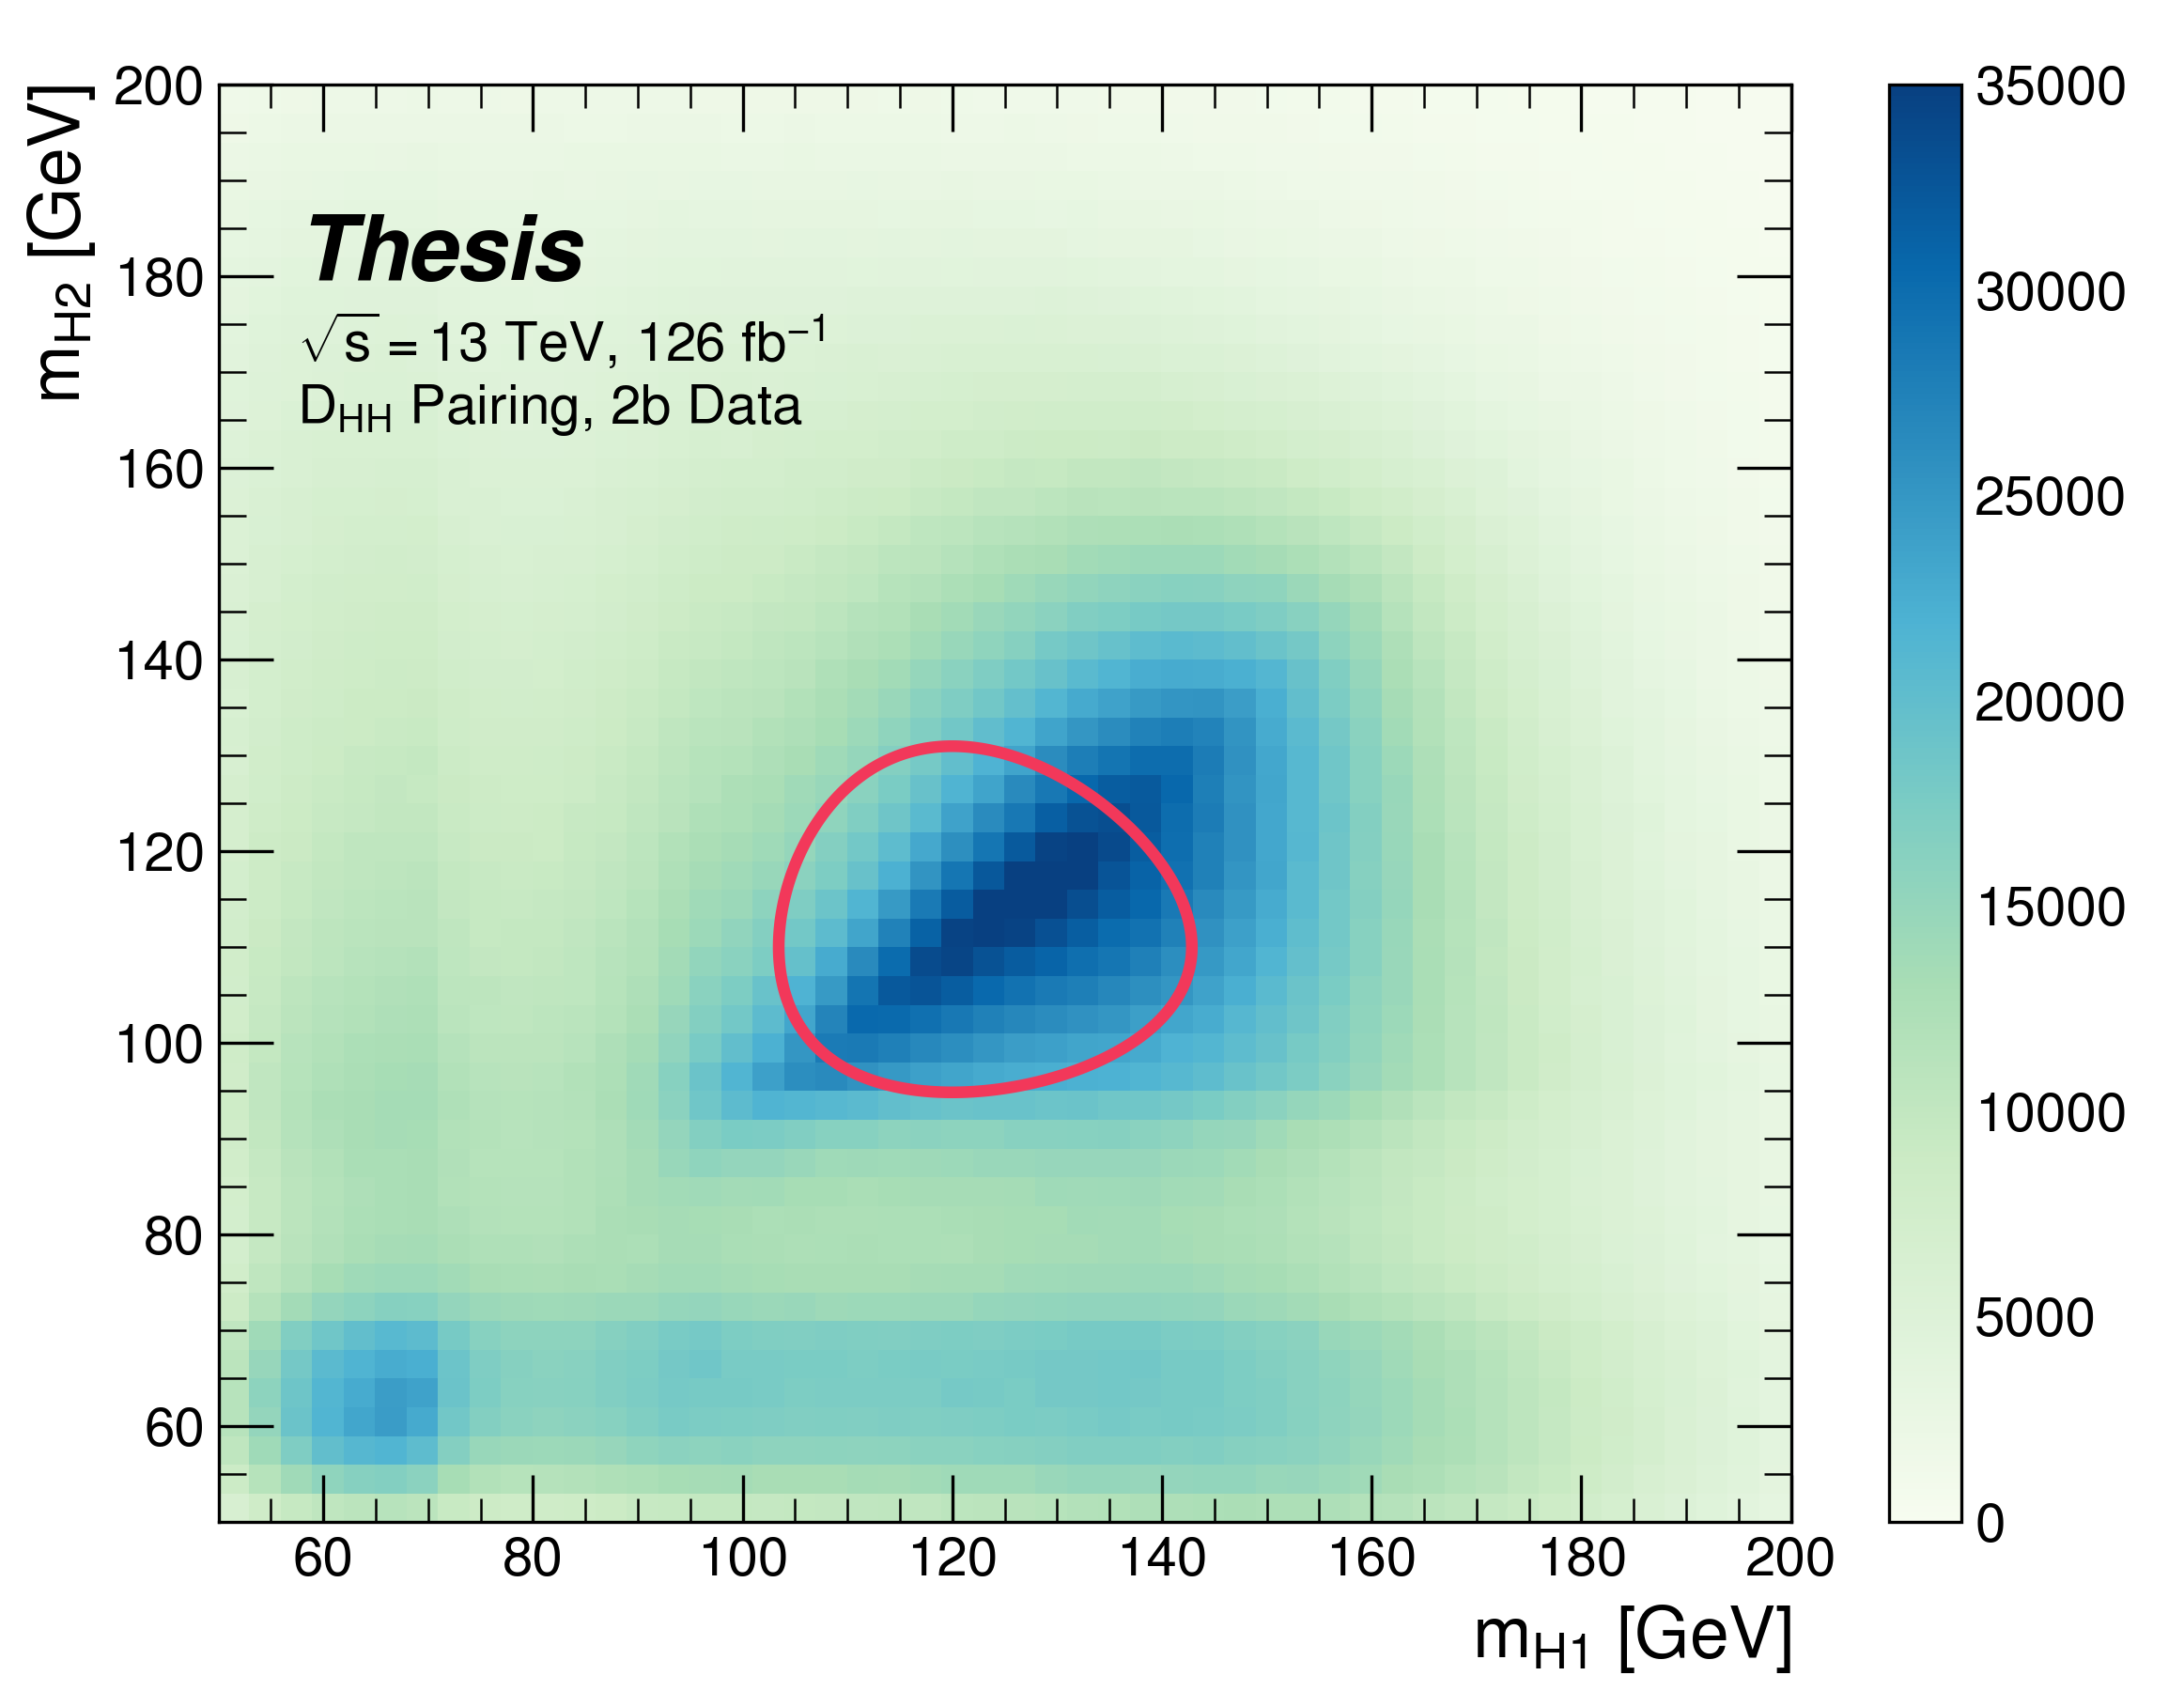
\includegraphics[width=0.48\textwidth]{figures/DHH-pairing-2b-massplane.png}
		 }
\caption{\label{fig:pairing-massplanes} Comparison of $m_{H1}$ vs $m_{H2}$ planes for the full Run 2 $2b$ 
dataset with different pairings, where $m_{H1}$ and $m_{H2}$ are the invariant masses of the leading and 
subleading Higgs candidates. As evidenced, this choice significantly impacts where events 
fall in this plane, and therefore which events fall into the various kinematic regions defined in 
this plane (see Section \ref{sec:kinematic-reg}). The signal regions for the resonant/early Run 2 analysis 
are shown for reference for the BDT and $D_{HH}$ pairings, while the the $\min\Delta R$ signal region shifted 
is shifted slightly up and to the right to match the non-resonant 
selection. Note that the band structure around \SI{80}{\GeV} in both $m_{H1}$ and $m_{H2}$ is introduced 
by the top veto described in Section \ref{sec:kinematic-cuts}.}
\end{figure}


\begin{figure}[ht]

\centering
\subfloat[$\kappa_{\lambda} = 1$ (SM)]{\label{fig:mindR-Dhh-sig-kl1}
		  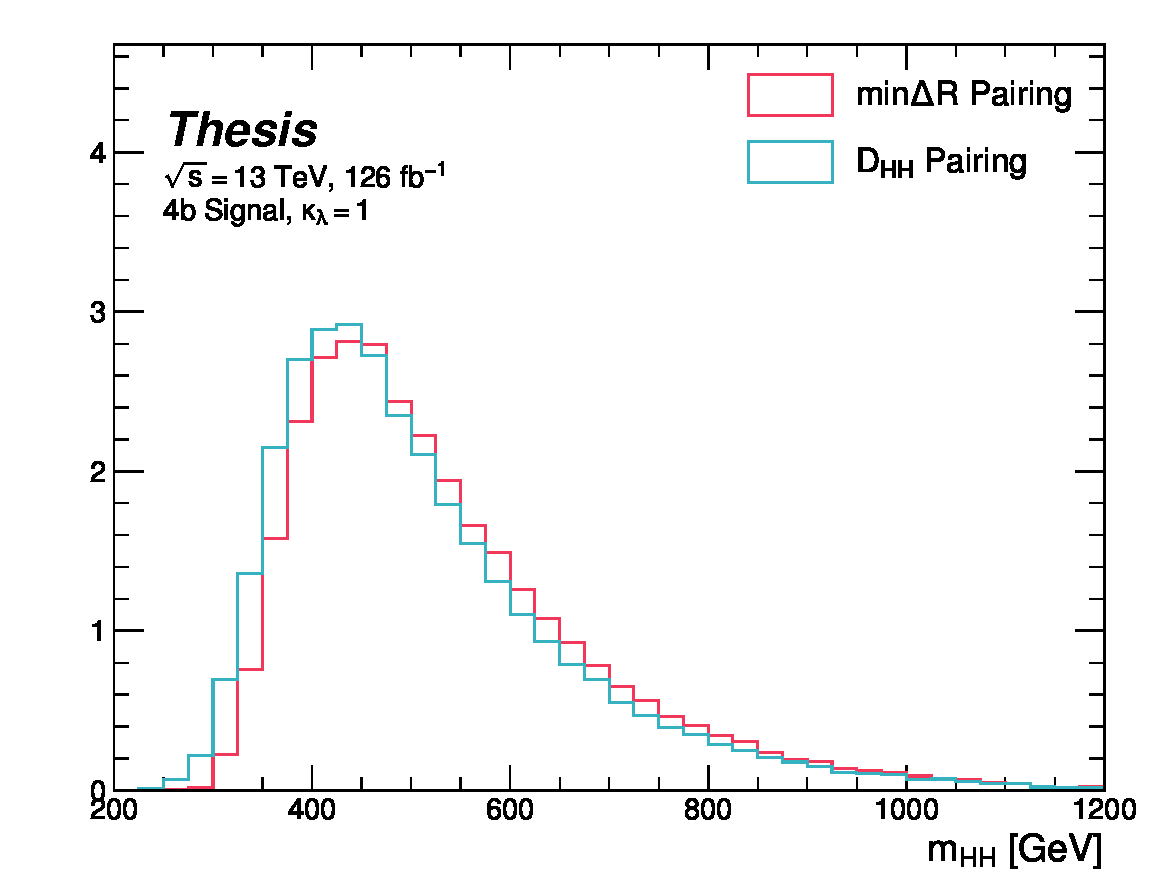
\includegraphics[width=0.48\textwidth]{figures/mindR-vs-Dhh-kl-1.pdf}
		 }
\subfloat[$\kappa_{\lambda} = -10$]{\label{fig:mindR-Dhh-sig-kl--10}
		  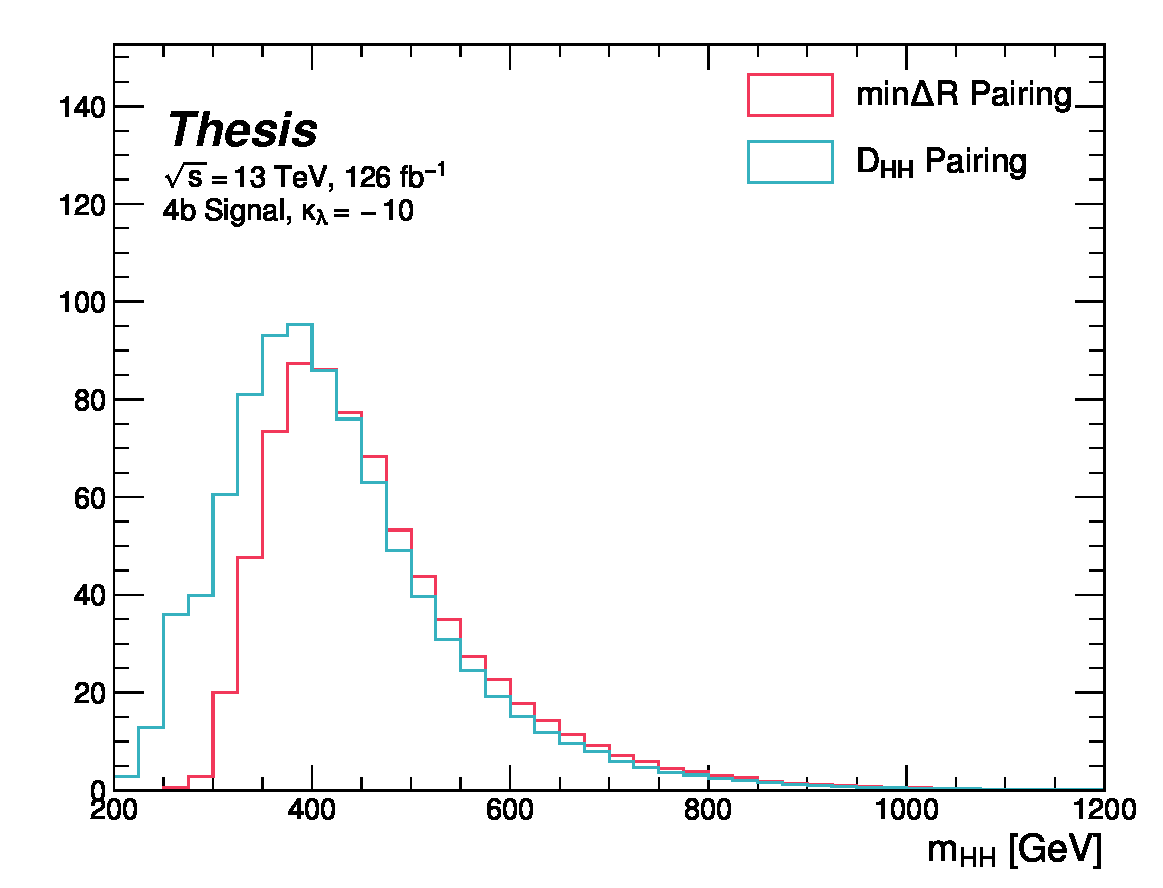
\includegraphics[width=0.48\textwidth]{figures/mindR-vs-Dhh-kl--10.pdf}
		 }

\subfloat[$\kappa_{\lambda} = 3$]{\label{fig:mindR-Dhh-sig-kl-3}
		  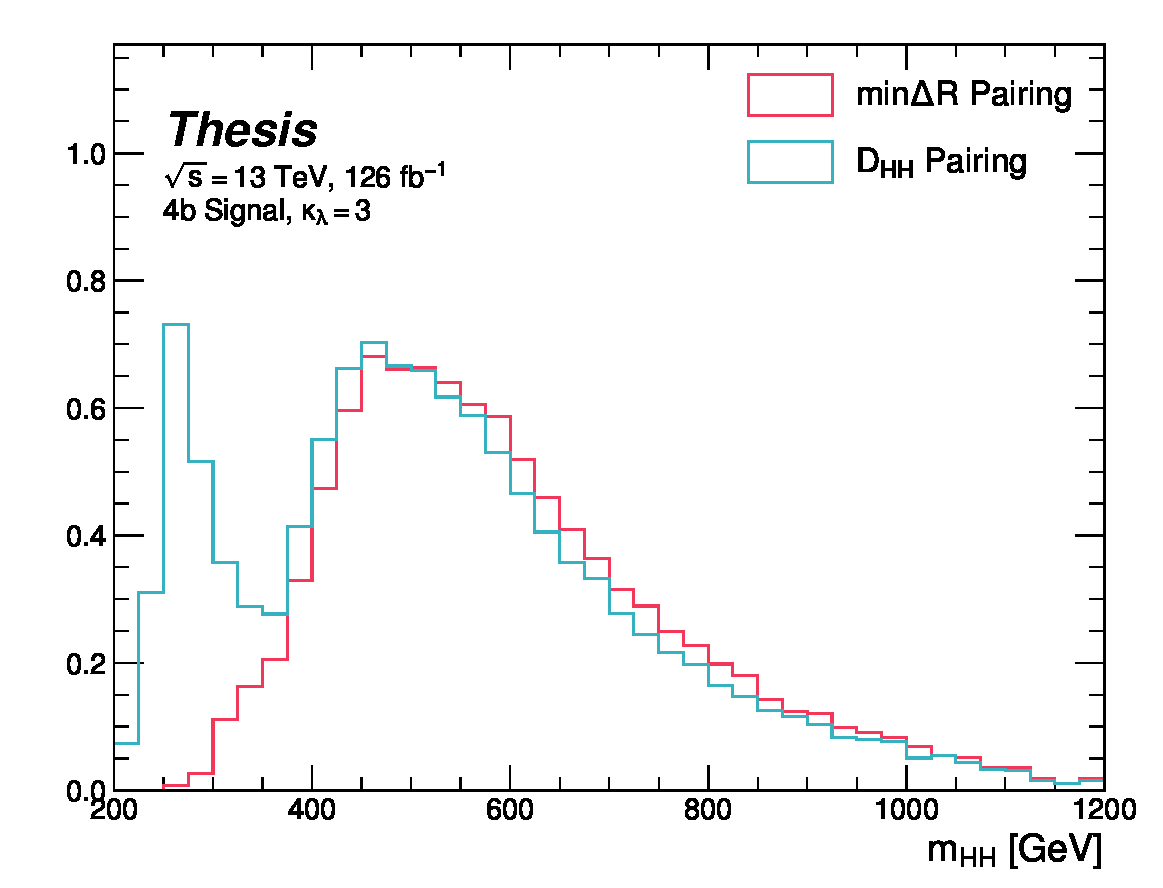
\includegraphics[width=0.48\textwidth]{figures/mindR-vs-Dhh-kl-3.pdf}
		 }
\subfloat[$\kappa_{\lambda} = 10$]{\label{fig:mindR-Dhh-sig-kl-10}
		  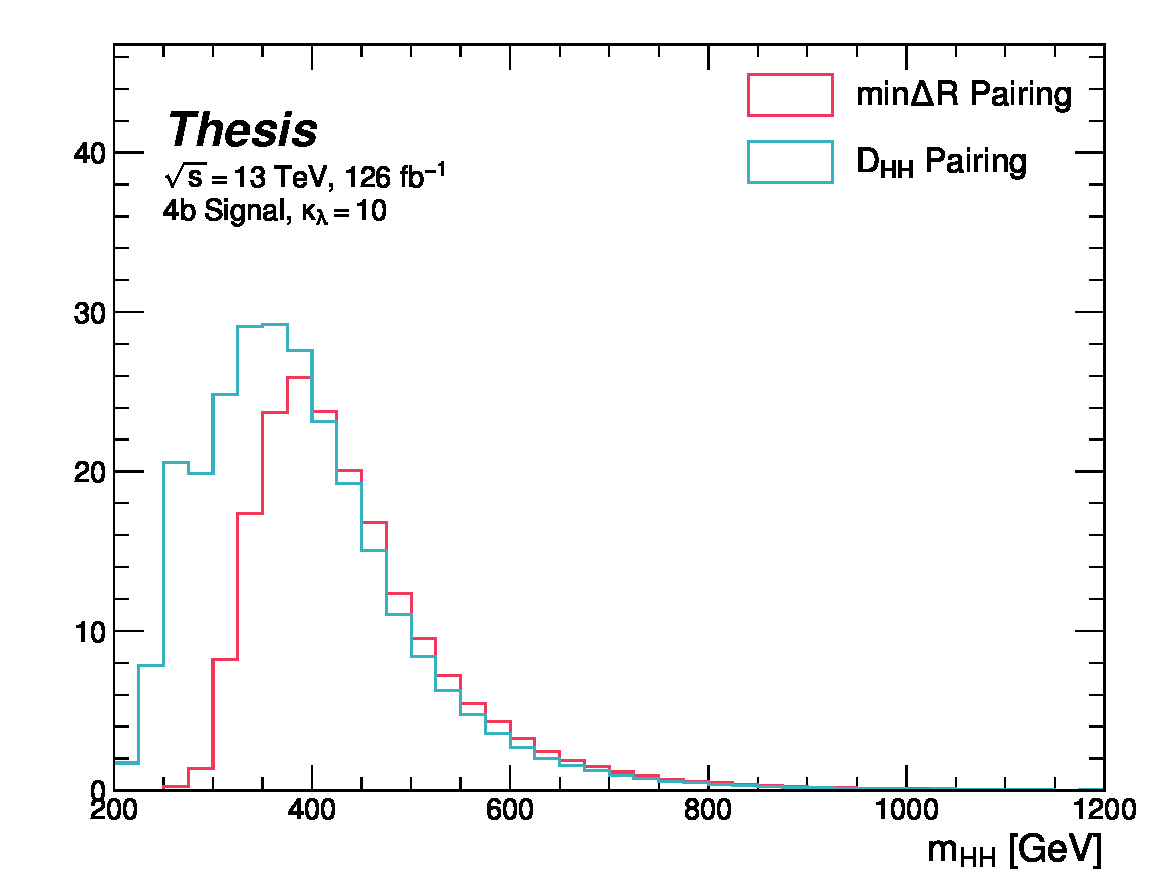
\includegraphics[width=0.48\textwidth]{figures/mindR-vs-Dhh-kl-10.pdf}
		 }
\caption{\label{fig:pairing-signal} 
Comparison of signal distributions in the respective signal regions for the $\min\Delta R$ and 
$D_{HH}$ pairing for various values of the Higgs trilinear coupling. The 
distributions are quite similar at the Standard Model point, but for other variations, $\min\Delta R$ does not 
pick up the low mass features.}
\end{figure}


\subsection{Resonant Pairing Strategy}

For the resonant analysis, a Boosted Decision Tree (BDT) is used for the pairing.
The boosted decision tree is given the total separation between the two jets in
each of the two pairs ($\Delta R_{1}$ and $\Delta R_{2}$), the pseudo-rapidity
separation between the two jets in each pair ($\Delta \eta_{1}$ and
$\Delta \eta_{2}$), and the angular separation between the two jets in each pair
in the $x$~--~$y$ plane ($\Delta \phi_{1}$ and $\Delta \phi_{2}$). The total
separations ($\Delta R$s) are provided in addition to the components in order to
avoid requiring the boosted decision tree to reconstruct these variables in
order to use them. For these variables, pair 1 is the pair with the highest
scalar sum of jet \pt{}s, and pair 2 the other pair.

The boosted decision tree is also parameterized on the di-Higgs mass (\mhh)
by providing this as an additional feature. Since the boosted decision tree is
trained on correct and incorrect pairings in signal events, there will be exactly one
correct pairing and two incorrect pairings in the training set for each \mhh
value present in that set. As a result, this variable cannot, in itself,
distinguish a correct pairing from an incorrect pairing, and therefore the
inclusion of this variable simply serves to parameterize the BDT on
\mhh\footnote{That is, the conditions placed on the other variables by the BDT
	vary with \mhh.}.

The boosted decision tree was trained on one quarter of the total AFII
simulated scalar MC statistics, using the Gradient-based One Side Sampling
(GOSS) algorithm which allows rapid training with very large datasets. A
preselection was applied requiring events to have four jets with a \pt of at
least \SI{35}{\GeV}. Note that this is a looser requirement than the
\SI{40}{\GeV} used in the analysis selection, and is meant to increase the
available statistics for events with low \mhh and to ensure a better
performance as a function of that variable. Events were also required to have
four distinct jets that could be geometrically matched (to within
$\Delta R \leq 0.4$) to the \bquarks. The events used to train the BDT were
not included when the analysis was run on these signal simulations. The
boosted decision tree was constructed with the following hyperparameters:\\
\code{min_data_in_leaf=50,\\
	num_leaves=180,\\
	learning_rate=0.01}

These hyperparameters were optimized using a Bayesian optimization
procedure~\cite{skopt}. Three fold cross-validation was used to perform this
optimization without the need for an additional sample, while avoiding
over-training on signal events.

\subsection{Non-resonant Pairing Strategy}
For the non-resonant analysis, a simpler pairing algorithm is used, which 
proceeds as follows: in a given event, Higgs candidates for each possible pairing
are sorted by the $p_{T}$ of the vector sum of constituent jets. The angular separation,
$\dr$ is computed between jets in the each of the leading Higgs candidates, and the 
pairing with the smallest separation ($\dr_{jj}$) is selected. This method will be 
referred to as $\min{\dr}$ in the following.

The primary motivation for the use of this pairing in the non-resonant search is a 
\emph{smooth mass plane}: by efficiently discarding low mass events, $\min{\dr}$ removes 
the background peak present in the resonant search while maintaining good pairing 
efficiency for the Standard Model non-resonant signal. This facilitates a background estimate with 
small kinematic bias -- the region in which the background estimate is derived is 
more similar to the signal region. 

Along with discarding low mass background, there is a corresponding loss of low mass signal.
This predominantly impacts points away from the Standard Model (see Figure \ref{fig:pairing-signal}), 
but, because the $4b$ channel has the strongest contribution near the Standard Model and because of the 
large low mass background present with other pairing methods, the impact on analysis sensitivity 
is mitigated. The $\min{\dr}$ pairing is thus adopted for the non-resonant search.

\subsection{Pairing Efficiencies}
Though this is implicit in the above descriptions, an explicit examination of the pairing 
efficiencies with respect to truth for the respective signal samples has been performed for both 
$\min{\Delta R}$ and the BDT pairing. Conceptually, for high invariant mass of the $HH$ system, 
each Higgs has a high $p_{T}$ and the the $b$-jets corresponding to a given Higgs are more collimated. 
In this case, angular information such as that exploited both directly by $\min{\Delta R}$ and as inputs in 
the BDT pairing may be expected to be a good discriminant for determining the $HH$ system. Indeed 
for resonance masses above \SI{500}{\GeV}, the pairing efficiency for both algorithms is close to 
100~\%.

For lower $HH$ masses, the jets corresponding to a given Higgs are no longer as collimated, such that 
$\min{\Delta R}$ is no longer guaranteed to pick up the correct pairing (e.g. in a case when the four jets 
involved are isotropic), and the pairing efficiency steadily gets worse as the $HH$ mass decreases. On 
resonant samples, e.g., the $\min{\Delta R}$ efficiency drops below 80~\% near \SI{400}{\GeV}. 
The additional information exploited by the BDT mitigates this somewhat, though there is still a drop 
in efficiency at lower $m_{HH}$. Interestingly, the BDT pairing demonstrates a 
rise in pairing efficiency near the threshold of \SI{250}{\GeV}, likely due to the limited kinematic 
phase space for the $HH$ system in this region.

The examination of the pairing efficiency as a function of $m_{HH}$ has a more direct correspondence for 
resonant samples, but it of course applies to non-resonant samples as well, resulting in the behavior shown 
in Figure \ref{fig:pairing-signal}. Note that the above statement 
that $\min{\dr}$ discards low mass events is a consequence of the reduced pairing efficiency at low mass -- 
the pairing algorithm itself does not make any cuts, but the mis-reconstruction of low mass signal results 
in the reconstruction of Higgs candidates with masses away from \SI{125}{\GeV}, placing such events outside of 
the kinematic signal regions defined in Section \ref{sec:kinematic-reg}.

\FloatBarrier
\clearpage
\section{Background Reduction and Top Veto}
\label{sec:kinematic-cuts}

Choosing a pairing of the four b-tagged jets fully defines the di-Higgs candidate system used for each event in the remainder of the analysis chain. A requirement of
$\abs{\Delta\eta_{\higgs\higgs}} < 1.5$ on this di-Higgs candidate system mitigates
QCD multijet background.

In order to mitigate the hadronic \ttbar background, a top veto is then applied,
removing events consistent with a \HepProcess{\Pqt \to \Pqb (\PW \to \Pq_{1} \Paq_{2})}
decay.

The jets in the event are separated into \emph{HC jets} which are
the four jets used to build the Higgs candidates, and \emph{non-HC jets}, the
other jets (passing the \pt and $\abs{\eta}$ requirements) in the event.

\PW candidates are built by forming all possible pairs of all jets in each event.
With $n$ jets, there are $\binom{n}{2}$ such pairs. \Pqt candidates are then built
by pairing each \PW candidate with each HC jet (for $4\binom{n}{2}$ combinations).
Note that all jets in a \Pqt candidate must be distinct (i.e. a HC jet may not be
used both on its own and in a \PW candidate).

With $m_{\Pqt}$ denoting the invariant mass of the \Pqt candidate, and $m_{\PW}$
the invariant mass of the \PW candidate, the quantity
\begin{equation}
	\label{eqn:xwt-def}
	X_{\PW\Pqt} = \sqrt{\qty(\frac{m_{\PW} - \SI{80.4}{\GeV}}{0.1\cdot m_{\PW}})^{2} + \qty(\frac{m_{\Pqt} - \SI{172.5}{\GeV}}{0.1\cdot m_{\Pqt}})^{2}}
\end{equation}

is constructed for each combination.

Events are then vetoed if the minimum $X_{\PW\Pqt}$ over all combinations is
less than 1.5.

The same definitions and procedures are used for both the resonant and non-resonant analyses.
However, for the non-resonant search, the top candidates considered for $X_{\PW\Pqt}$ have the 
additional requirement that the jet used for the $b$ is $b$-tagged. While this is identical
to the resonant analysis by definition for $4b$ events, it does change the set of events 
considered in lower tag regions, in particular for the $2b$ events considered in the derivation
of the background estimate. Such a change is found to reduce the impact of background systematics, an 
effect that is thought to be due to the shifting of $2b$ events to higher values of $X_{\PW\Pqt}$ (due to 
this more stringent requirement), where, e.g, the Standard Model signal peaks.

The distribution of this variable is shown for $t\bar{t}$ Monte Carlo and representative signal 
samples for the resonant and non-resonant $4b$ signal regions in Figures \ref{fig:Xwt-res} and 
\ref{fig:Xwt-nonres} respectively, with a line at the cut value of 1.5. Individual years are shown, 
but results are representative across years. For the resonant analysis, the value of the cut is 
constrained by low mass resonances, with the value of 1.5 chosen as a compromise between $t\bar{t}$ 
rejection and retaining sensitivity for these signals. For the non-resonant, though e.g., the SM signal 
peaks at higher values, a more aggressive cut on $X_{Wt}$ was found to decrease analysis sensitivity, 
so the value of 1.5 is kept.
\begin{figure}
\centering
\subfloat{
		  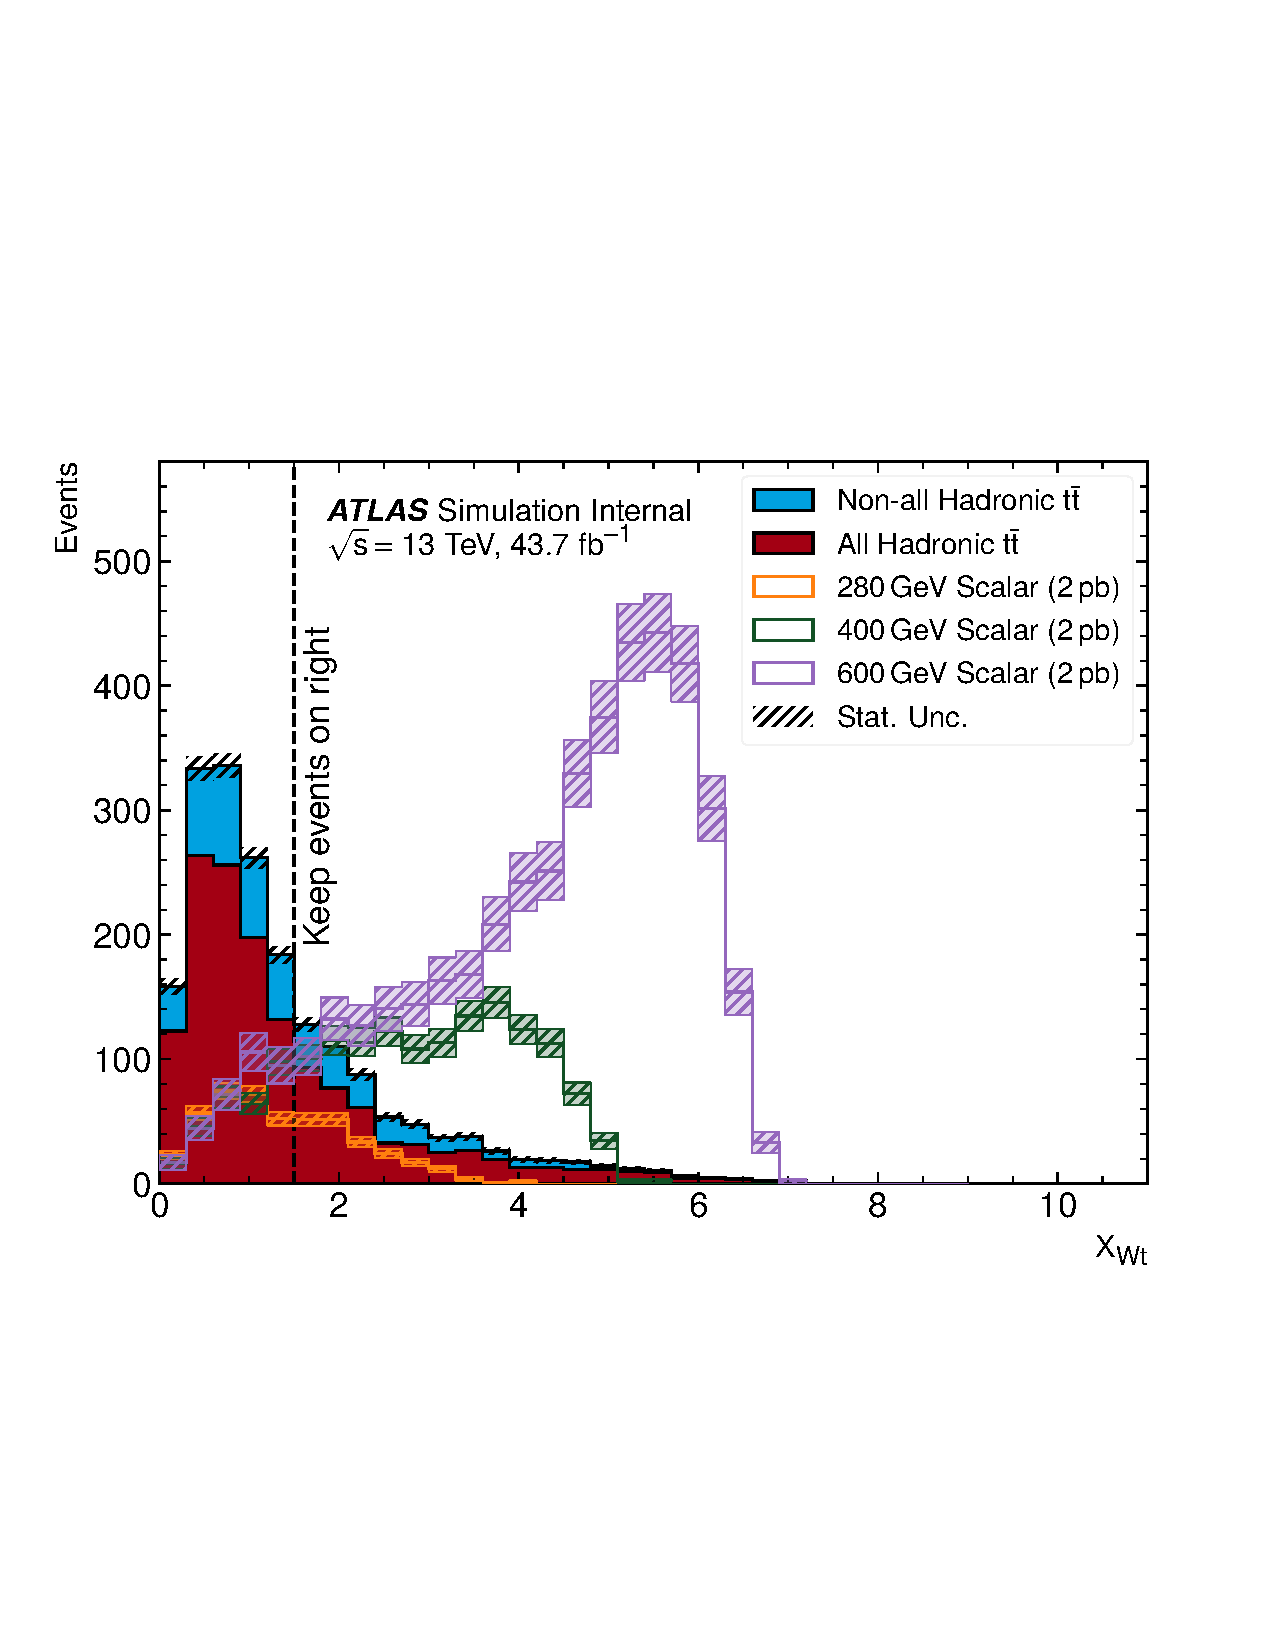
\includegraphics[width=0.8\textwidth]{figures/Xwt-res.pdf}
  }
\caption{\label{fig:Xwt-res} \textbf{Resonant search}: Illustration of the impact of the top veto on $t\bar{t}$ 
Monte Carlo for the resonant analysis, with representative scalar signals shown for reference. The cut value 
used is 1.5, shown in the dashed black, and events below this value are discarded. This top veto clearly removes 
the bulk of $t\bar{t}$ events, and the value of the cut is chosen to retain analysis sensitivity, particularly for 
low mass.}
\end{figure}

\begin{figure}
\centering
\subfloat{
		  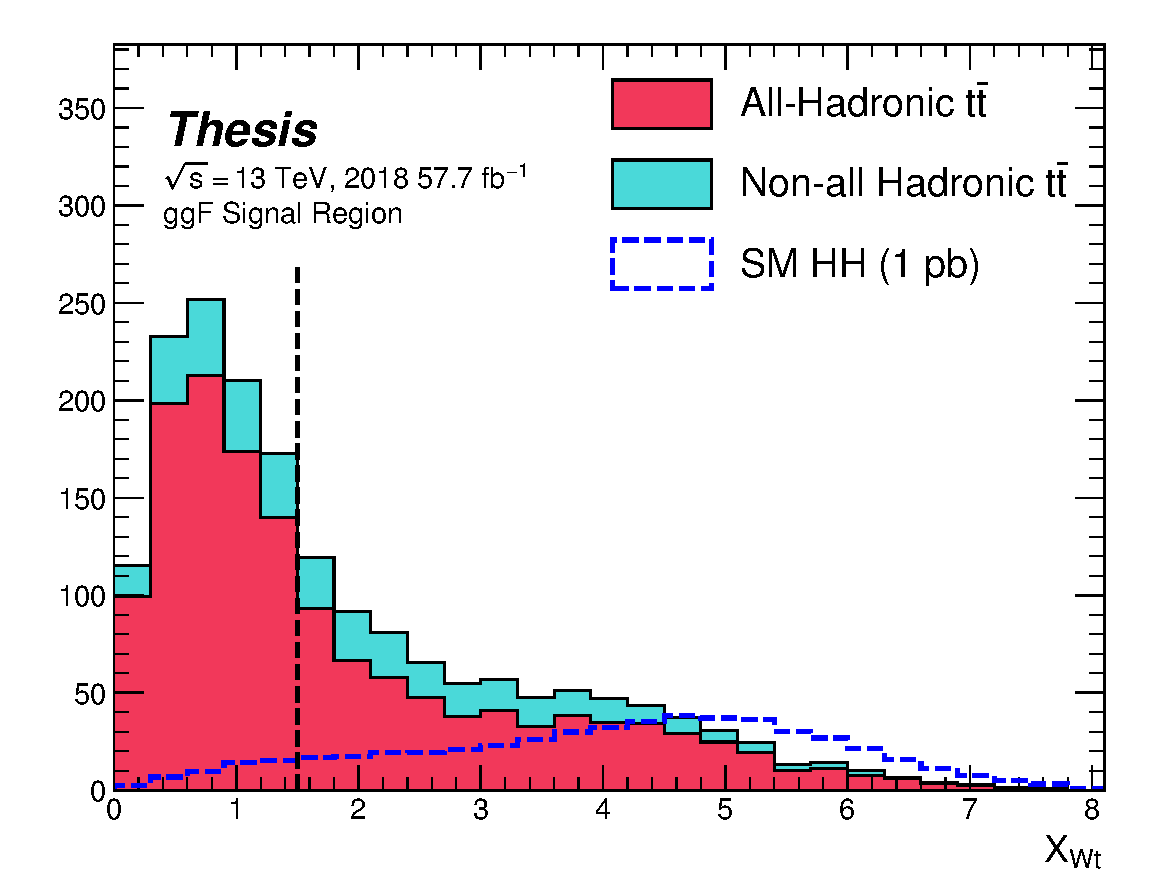
\includegraphics[width=0.8\textwidth]{figures/Xwt-nonres.pdf}
  }
\caption{\label{fig:Xwt-nonres} \textbf{Non-resonant search}: Illustration of the impact of the top veto on $t\bar{t}$ 
Monte Carlo for the non-resonant analysis, with the Standard Model signal shown for reference. The cut value 
used is 1.5, shown in the dashed black, and events below this value are discarded. This top veto clearly removes 
the bulk of $t\bar{t}$ events. While this plot may seem to motivate a more aggressive cut on $X_{Wt}$, increasing 
the value of the cut was found to reduce analysis sensitivity.}
\end{figure}



\FloatBarrier
\clearpage
\section{Kinematic Region Definition}
\label{sec:kinematic-reg}
As has been mentioned, an important piece of the analysis is the plane defined by the 
two Higgs candidate masses (the \emph{Higgs candidate mass plane}). After the selection
described above, a signal region is defined by requiring $X_{\higgs\higgs} < 1.6$, where:
\begin{equation}
	\label{eqn:xhh-def}
	X_{\higgs\higgs} = \sqrt{\qty(\frac{\mh1 - c_1}{0.1\cdot\mh1})^{2} + 
	\qty(\frac{\mh2 - c_2}{0.1\cdot\mh2})^{2}}
\end{equation}
with \mh1, \mh2 the leading and subleading Higgs candidate masses, $c_{1}$ and $c_{2}$ correspond
to the center of the signal region, and the denominator provides a Higgs candidate mass 
dependent resolution of 10~\%. For consistency with the $HH$ decay hypothesis, $c_{1}$ and $c_{2}$
are nominally (\SI{125}{\GeV}, \SI{125}{\GeV}). However, these are allowed to vary due to 
energy loss, with specific values chosen described below. The selection of these values is 
one of several significant differences between the regions defined for the resonant and non-resonant search.
We describe both below.

\subsection{Resonant Kinematic Regions}
For the resonant analysis, the signal region is centered at (\SI{120}{\GeV}, \SI{110}{\GeV}) 
to account for energy loss leading to the Higgs masses being under-reconstructed. Note that leading and 
subleading Higgs candidates are defined according to the 
\emph{scalar sum} of constituent jet $p_{T}$.

For the background estimation, two regions are defined which are roughly concentric around the 
signal region: a \emph{validation region} which 
consists of those events not in the signal region, but which do pass
\begin{equation}
	\label{eqn:val-reg-def}
	\sqrt{\qty(\mh1 - 1.03 \times \SI{120}{\GeV})^{2} + \qty(\mh2 - 1.03 \times
		\SI{110}{\GeV})^{2}} < \SI{30}{\GeV}
\end{equation}
and a \emph{control region} which consists of those events not in the signal or validation
regions, but which do pass
\begin{equation}
	\label{eqn:ctrl-reg-def}
	\sqrt{\qty(\mh1 - 1.05 \times \SI{120}{\GeV})^{2} + \qty(\mh2 - 1.05 \times
		\SI{110}{\GeV})^{2}} < \SI{45}{\GeV}
\end{equation}

For simplicity, the SR/VR/CR definitions from the early Run 2 paper~\cite{EXOT-2016-31} were chosen 
for the resonant analysis, and were found to be close to optimal. These regions are shown in Figure 
\ref{fig:res-regions}.

\begin{figure}
\centering
\subfloat{
		  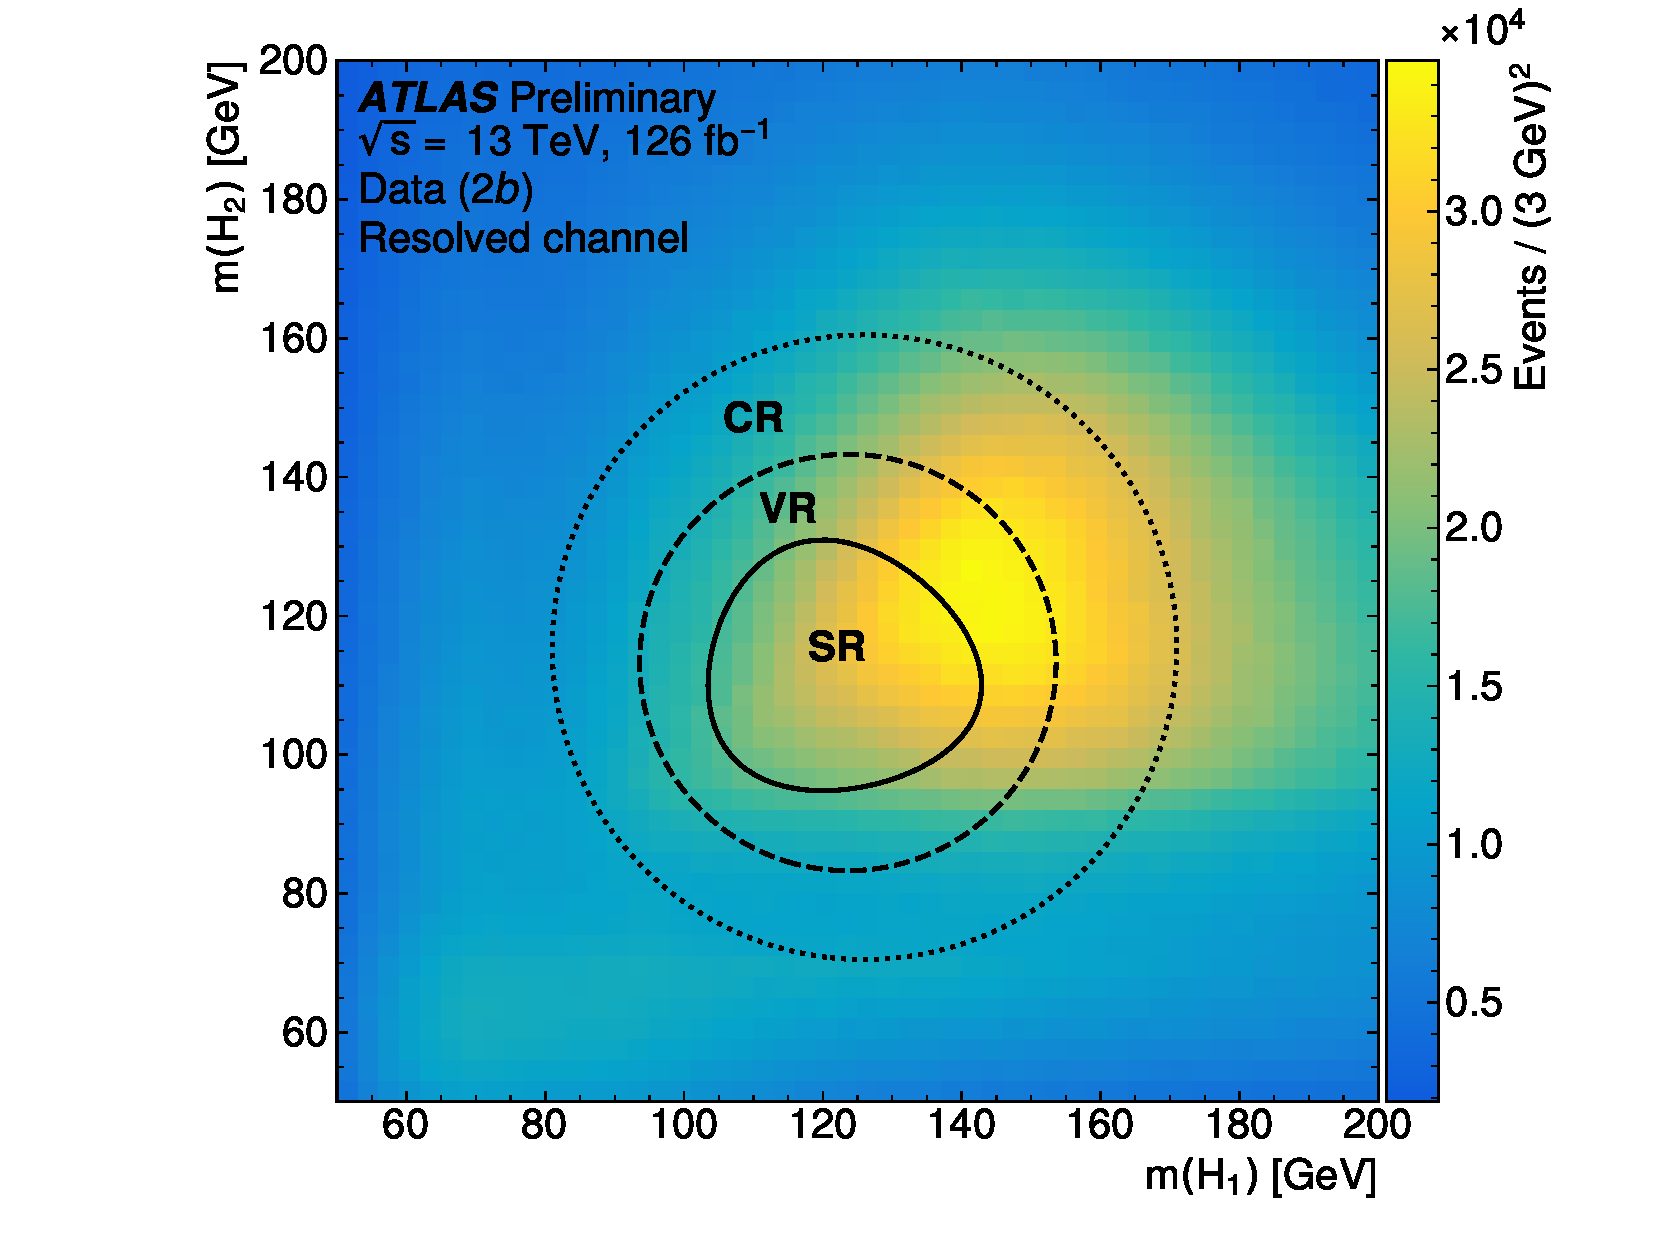
\includegraphics[width=0.8\textwidth]{figures/region-def-resolved.pdf}
  }
\caption{\label{fig:res-regions} Regions used for the resonant search, shown on the $2b$ data  
mass plane. The outermost region (the ``control region'') is used for derivation of the nominal 
background estimate. The innermost region is the signal region, where the signal extraction 
fit is performed. The region in between (the ``validation region'') is used for the assessment of an 
uncertainty.}
\end{figure}

\subsection{Non-resonant Kinematic Regions}
For the non-resonant analysis the signal region is centered at (\SI{124}{\GeV}, \SI{117}{\GeV}),
corresponding to the means of \emph{correctly paired} Standard Model signal events. The shape of 
the signal region (other than this change of center) was found to remain optimal.

For the non-resonant search, leading and subleading Higgs candidates are defined according to the 
\emph{vector sum} of constituent jet $p_{T}$, more closely corresponding to the $1\rightarrow 2$ decay assumption
behind the $\min{\dr}$ pairing algorithm. 

Two areas for improvement were identified in the resonant analysis, which will be discussed in more detail below: 
\emph{signal contamination} of the validation region (which impacts the uncertainty assessed due to extrapolation)
and \emph{large nuisance parameter pulls} for this uncertainty, corresponding to a rough assumption that the 
validation region is closer to the signal region in the mass plane, and so offers a better estimate of the 
signal region. Extensive cross-checks were performed for the resonant search, which demonstrated minimal 
bias due to the signal contamination and healthy behavior of the signal extraction fit, despite 
the large pulls. However, these large pulls imply that the nominal estimate may be improved by 
incorporating some of the information entering the definition of the extrapolation uncertainty. Further, 
the resonant search benefits from a set of highly peaked signals, such that the smooth nature of the 
background helps to mitigate signal contamination bias. With the broad non-resonant signals, 
a bias due to signal contamination becomes more of a concern, such that addressing this is highly 
motivated.

A redesign of the control and validation regions is therefore performed for 
the non-resonant analysis. The outer boundary defined by the shifted resonant control region:
\begin{equation}
	\label{eqn:ctrl-reg-def}
	\sqrt{\qty(\mh1 - 1.05 \times \SI{124}{\GeV})^{2} + \qty(\mh2 - 1.05 \times
		\SI{117}{\GeV})^{2}} < \SI{45}{\GeV}
\end{equation}
is kept, roughly corresponding to combining the regions used for the resonant analysis. In order 
to assess the variation of the background estimate, two sets of regions are desired, so this combined 
region is split into \emph{quadrants}, that is, divided into four pieces along axes that intersect 
with the signal region center. To avoid kinematic bias, quadrants on opposite sides of the signal 
region are paired, with these pairs corresponding to the non-resonant control and validation regions.

The particular orientation of the regions is chosen such that region centers align with the leading
and subleading Higgs candidate masses, corresponding to a set of axes rotated at $45^{\circ}$, with the ``top''
and ``bottom'' quadrants together comprising the control region, and the other set (``left'' and ``right'')
the validation region. These regions are shown in Figure \ref{fig:nonres-regions}
\begin{figure}
\centering
\subfloat{
		  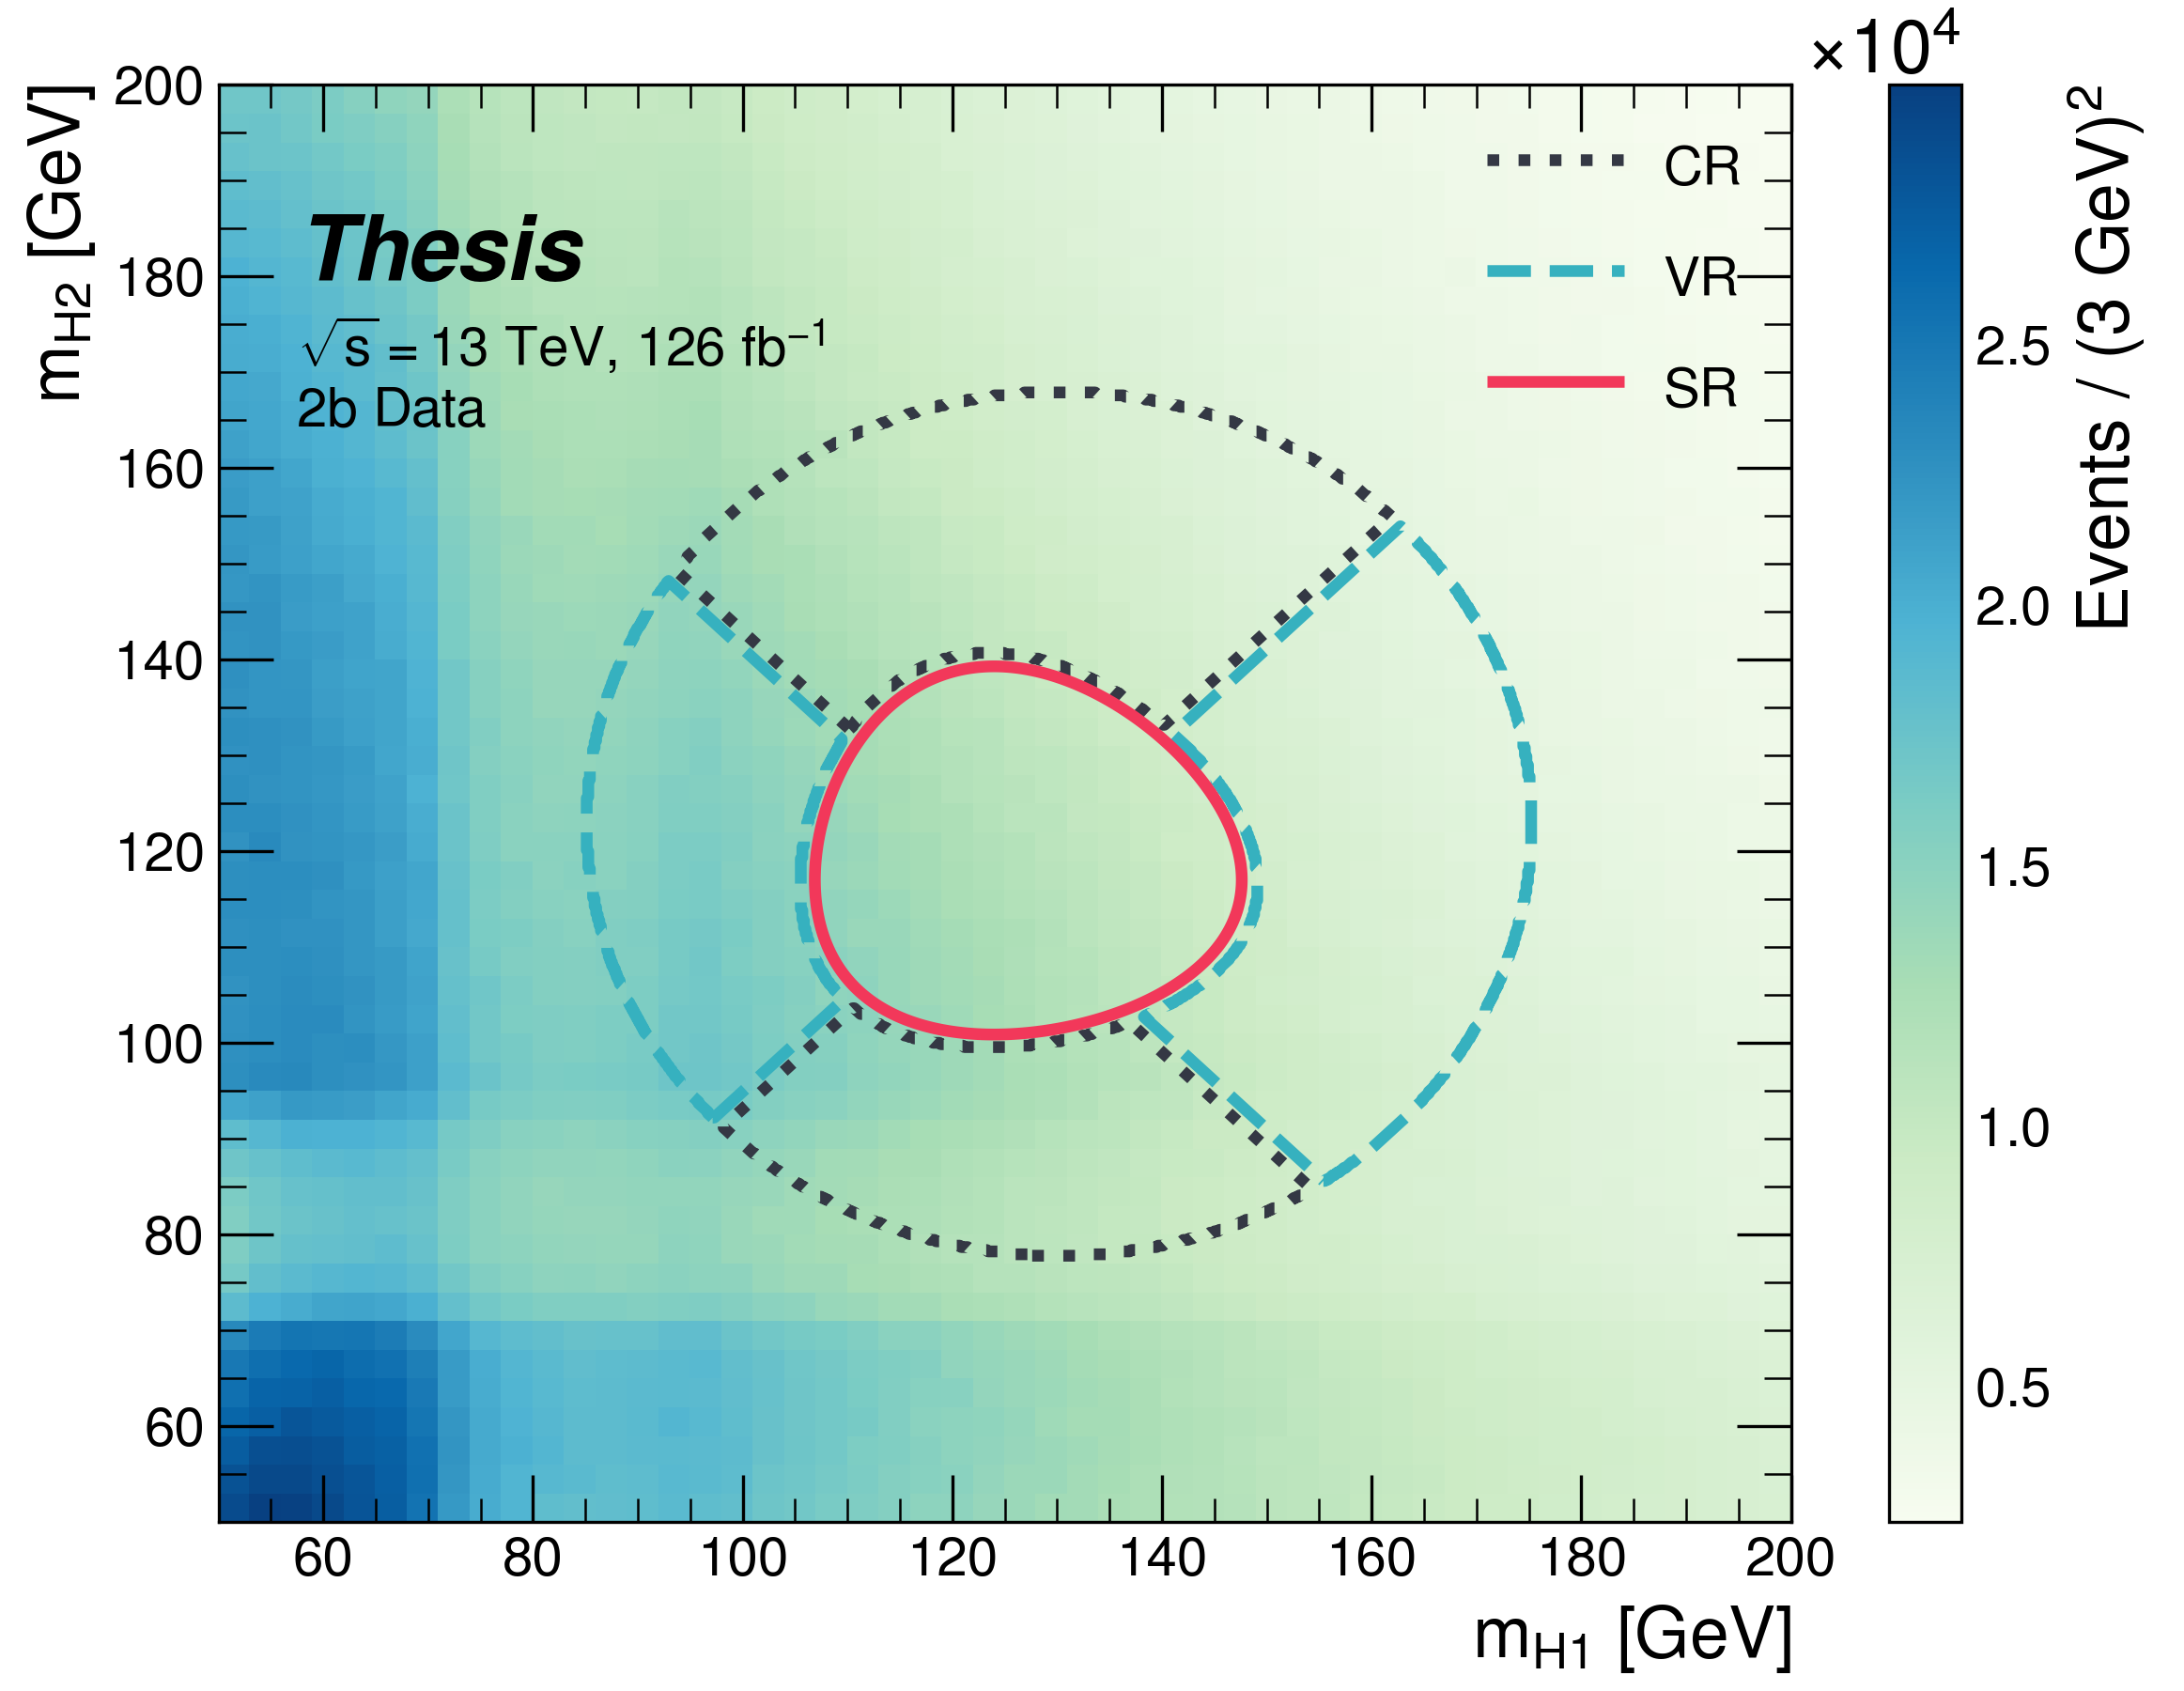
\includegraphics[width=0.8\textwidth]{figures/nonres-regions.png}
  }
\caption{\label{fig:nonres-regions} Regions used for the non-resonant search. The ``top''
and ``bottom'' quadrants together comprise the control region, in which the nominal background 
estimate is derived. The``left'' and ``right'' quadrants together comprise the validation region, 
which is used to assess an uncertainty. The signal region, in the center, is where the signal extraction 
fit is performed.}
\end{figure}

This design of regions includes a set of events closer to the signal region in the mass plane, leveraging
the assumption that these events are more similar to signal region events, while also including events further away
from the signal region, mitigating signal contamination. This region selection is found to have good performance
in alternate validation regions (see Section \ref{sec:bkgd-validation}).

\subsection{Discriminating Variable}
\label{subsec:disc-var}

The discriminant used for the resonant analysis is \emph{corrected $m_{HH}$}. This
variable is calculated by re-scaling the Higgs candidate four vectors such that
each $m_{H} = \SI{125}{\GeV}$. These re-scaled four-vectors are then summed, and
their invariant mass is the corrected $m_{HH}$. These re-scaled four-vectors are
not used for any other purpose. The effect of this correction, which sharpens
the $m_{HH}$ peak and correctly centers it, is shown
in~\Fig{\ref{fig:m-hh-cor-effect}}.
\begin{figure}[ht]
\centering
\subfloat{
		  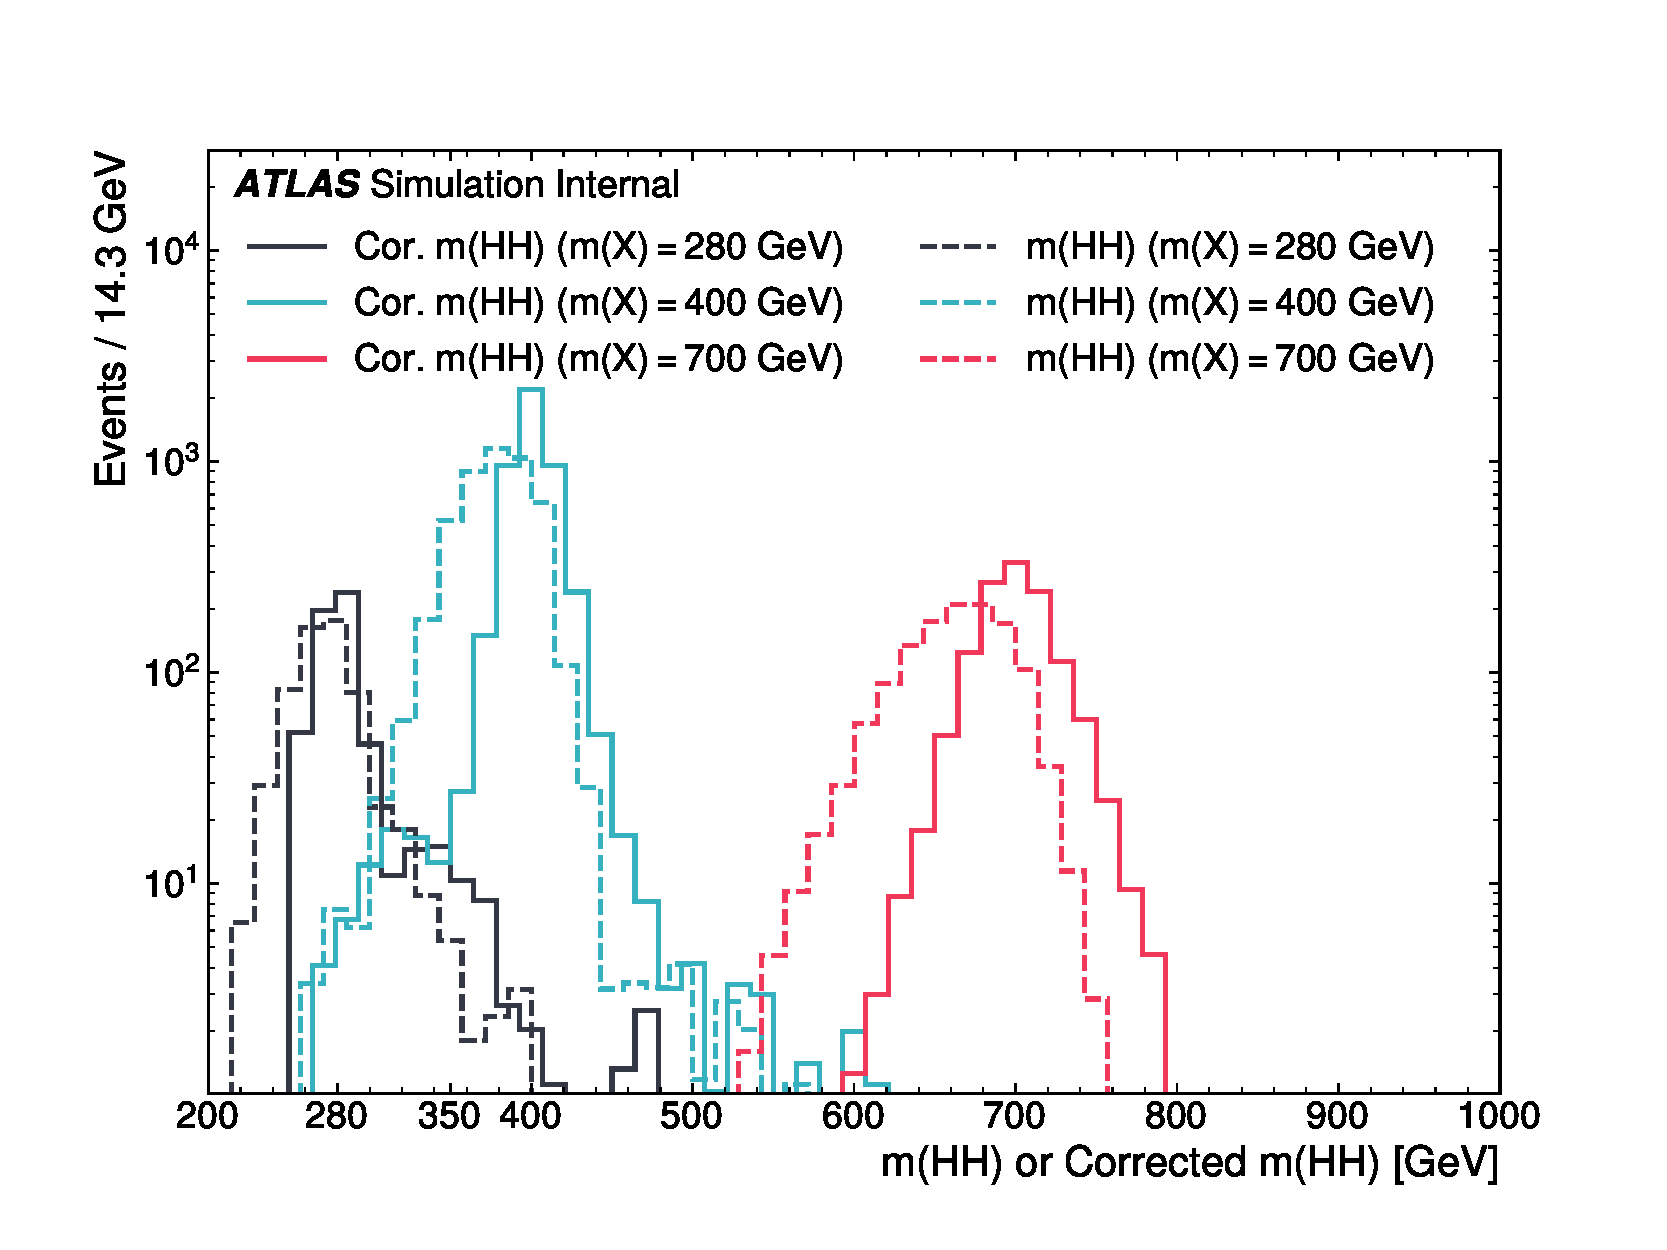
\includegraphics[width=0.8\textwidth]{figures/resolved-m-hh-cor.pdf}
  }
\caption{\label{fig:m-hh-cor-effect} Impact of the $m_{HH}$ correction on a range of spin-0 
resonant signals. The corrected $m_{HH}$ distributions (solid lines) are much sharper and 
more centered on the corresponding resonance masses than the uncorrected $m_{HH}$ distributions 
(dashed).}
\end{figure}

For the non-resonant analysis, due to the broad nature of the signal in \mhh, such a 
correction is not as motivated, and, indeed, is found to have very minimal 
impact. The uncorrected \mhh (just referred to as \mhh) is therefore used 
as a discriminant. To maximize sensitivity, the non-resonant analysis 
additionally uses two variables for categorization: $\Delta \eta_{HH}$, an angular 
variable which, along with \mhh, fully characterizes the $HH$ system~\cite{cosThetastar}, 
and $X_{HH}$, the variable used for the 
signal region definition, which leverages the peaked structure of the 
signal in the ($\mh1$, $\mh2$) plane to split the signal extraction fit into lower and higher
purity regions (highest purity near $X_{HH} = 0$, the center of the signal region).
Distributions of these variables are shown in \todo{plots}. The categorization used for this 
thesis has been optimized to be $2\times 2$ in these variables, with corresponding selections 
$0 \leq \Delta \eta_{HH} \leq 0.75$ and $0.75 \leq \Delta \eta_{HH} \leq 1.5$ for $\Delta \eta_{HH}$, 
and $0 \leq X_{HH} \leq 0.95$ and $0.95 \leq X_{HH} \leq 1.6$ for $X_{HH}$.
